\documentclass[11pt]{article} 
\usepackage[english]{babel}
\usepackage[utf8]{inputenc}
\usepackage[margin=0.5in]{geometry}
\usepackage{amsmath}
\usepackage{amsthm}
\usepackage{amsfonts}
\usepackage{amssymb}
\usepackage[usenames,dvipsnames]{xcolor}
\usepackage{graphicx}
\usepackage[siunitx]{circuitikz}
\usepackage{tikz}
\usepackage[colorinlistoftodos, color=orange!50]{todonotes}
\usepackage{hyperref}
\usepackage[numbers, square]{natbib}
\usepackage{fancybox}
\usepackage{epsfig}
\usepackage{soul}
\usepackage[framemethod=tikz]{mdframed}
\usetikzlibrary{positioning, automata, backgrounds}
\usepackage[shortlabels]{enumitem}
\usepackage[version=4]{mhchem}
\usepackage{multicol}
\usepackage{forest}
\usepackage{mathtools}
\usepackage{comment}
\usepackage{enumitem}
\usepackage[utf8]{inputenc}
\usepackage[linesnumbered,ruled,vlined]{algorithm2e}
\usepackage{listings}
\usepackage{color}
\usepackage[numbers]{natbib}
\usepackage{subfiles}
\usepackage{tkz-berge}


\newtheorem{prop}{Proposition}[section]
\newtheorem{thm}{Theorem}[section]
\newtheorem{lemma}{Lemma}[section]
\newtheorem{cor}{Corollary}[prop]

\theoremstyle{definition}
\newtheorem{definition}{Definition}

\theoremstyle{definition}
\newtheorem{required}{Problem}

\theoremstyle{definition}
\newtheorem{ex}{Example}


\newcommand{\interval}[4]{\draw (#2, #1) -- (#3, #1); % Usage: \interval{height}{start}{end}{label}
\draw (#2, #1-0.11) -- (#2, #1+0.11); % draw left whisker
\draw (#3, #1-0.11) -- (#3, #1+0.11); % draw right whisker
\node[] at (#2-0.25, #1) {#4};
}

\setlength{\marginparwidth}{3.4cm}
%#########################################################

%To use symbols for footnotes
\renewcommand*{\thefootnote}{\fnsymbol{footnote}}
%To change footnotes back to numbers uncomment the following line
%\renewcommand*{\thefootnote}{\arabic{footnote}}

% Enable this command to adjust line spacing for inline math equations.
% \everymath{\displaystyle}

% _______ _____ _______ _      ______ 
%|__   __|_   _|__   __| |    |  ____|
%   | |    | |    | |  | |    | |__   
%   | |    | |    | |  | |    |  __|  
%   | |   _| |_   | |  | |____| |____ 
%   |_|  |_____|  |_|  |______|______|
%%%%%%%%%%%%%%%%%%%%%%%%%%%%%%%%%%%%%%%

\title{
\normalfont \normalsize 
\textsc{CSCI 3104 Spring 2022 \\ 
Instructor: Profs. Chen and Layer} \\
[10pt] 
\rule{\linewidth}{0.5pt} \\[6pt] 
\huge Problem Set 3 \\
\rule{\linewidth}{2pt}  \\[10pt]
}
%\author{Your Name}
\date{}

\begin{document}
\definecolor {processblue}{cmyk}{0.96,0,0,0}
\definecolor{processred}{rgb}{200, 0, 0}
\definecolor{processgreen}{rgb}{0, 255, 0}
\DeclareGraphicsExtensions{.png}
\DeclareGraphicsExtensions{.gif}
\DeclareGraphicsExtensions{.jpg}

\maketitle


%%%%%%%%%%%%%%%%%%%%%%%%%
%%%%%%%%%%%%%%%%%%%%%%%%%%
%%%%%%%%%%FILL IN YOUR NAME%%%%%%%
%%%%%%%%%%AND STUDENT ID%%%%%%%%
%%%%%%%%%%%%%%%%%%%%%%%%%%
\noindent
Due Date \dotfill \textbf{February 8, 2022} \\
Name \dotfill \textbf{Chengming Li} \\
Student ID \dotfill \textbf{109251991} \\
Collaborators \dotfill \textbf{N/A}

\tableofcontents

\section{Instructions}
 \begin{itemize}
	\item The solutions \textbf{must be typed}, using proper mathematical notation. We cannot accept hand-written solutions. \href{http://ece.uprm.edu/~caceros/latex/introduction.pdf}{Here's a short intro to \LaTeX.}
	\item You should submit your work through the \textbf{class Canvas page} only. Please submit one PDF file, compiled using this \LaTeX \ template.
	\item You may not need a full page for your solutions; pagebreaks are there to help Gradescope automatically find where each problem is. Even if you do not attempt every problem, please submit this document with no fewer pages than the blank template (or Gradescope has issues with it).

	\item You are welcome and encouraged to collaborate with your classmates, as well as consult outside resources. You must \textbf{cite your sources in this document.} \textbf{Copying from any source is an Honor Code violation. Furthermore, all submissions must be in your own words and reflect your understanding of the material.} If there is any confusion about this policy, it is your responsibility to clarify before the due date. 

	\item Posting to \textbf{any} service including, but not limited to Chegg, Reddit, StackExchange, etc., for help on an assignment is a violation of the Honor Code.

	\item You \textbf{must} virtually sign the Honor Code (see Section \ref{HonorCode}). Failure to do so will result in your assignment not being graded.
\end{itemize}


\section{Honor Code (Make Sure to Virtually Sign)} \label{HonorCode}

\begin{required}
\begin{itemize}
\item My submission is in my own words and reflects my understanding of the material.
\item Any collaborations and external sources have been clearly cited in this document.
\item I have not posted to external services including, but not limited to Chegg, Reddit, StackExchange, etc.
\item I have neither copied nor provided others solutions they can copy.
\end{itemize}

%\noindent In the specified region below, clearly indicate that you have upheld the Honor Code. Then type your name. 
\end{required}

\begin{proof}[Agreed (signature here).]
%% Typing "I agree to the above," followed by your name is sufficient.
I agree to the above, Chengming Li
\end{proof}



\newpage
\section{Standard 7 - MST: safe and useless edges}

\begin{required}
Consider the weighted graph $G(V, E, w)$ below. Let $\mathcal{F} = \{ \{A, B\}, \{B, C\}, \{E, F\}\}$ be an intermediate spanning forest (indicated by the thick edges below). Label each edge that is \textbf {not} in $\mathcal{F}$ as safe, useless, or undecided. Provide a 1-2 sentence explanation for each such edge.


\begin{center}
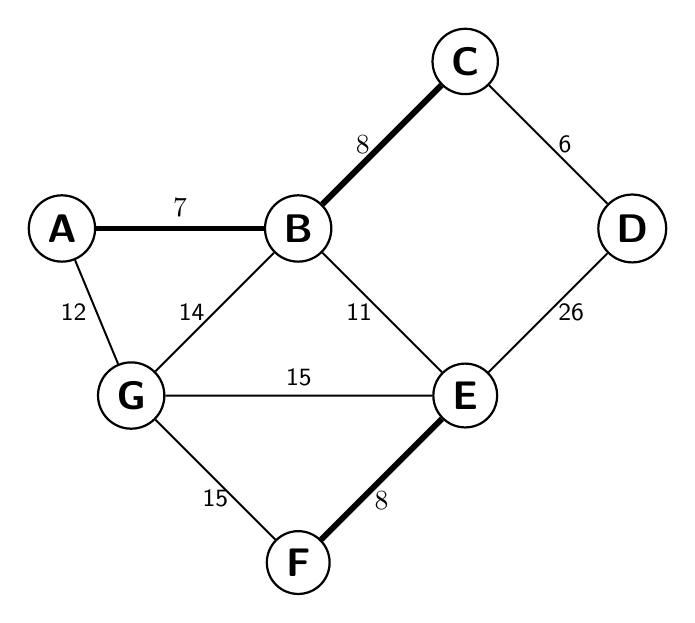
\begin{tikzpicture}[scale=0.4, auto, node distance=3cm, every loop/.style={},
  thick,main node/.style={circle,draw,font=\sffamily\Large\bfseries}]

\node[main node] (A) {A};
\node[main node] (B) [right of=A] {B};
\node[main node] (C) [above right of=B] {C};
\node[main node] (D) [below right of=C] {D};
\node[main node] (E) [below left of=D] {E};
\node[main node] (F) [below left of=E] {F};
\node[main node] (G) [above left of=F] {G};

\path[line width=0.25mm, every node/.style={font=\sffamily\small}]

(A) edge node [left]  {12} (G)
(B) edge node [left]  {11}  (E)
(C) edge node [right] {6}  (D)
(D) edge node [right] {26} (E)
(F) edge node [below] {15} (G)
(G) edge node [left]  {14} (B)
(G) edge node [above] {15}  (E)
;

\draw[line width=0.75mm] (A) -- node [above] {7} (B);
\draw[line width=0.75mm] (E) -- node [below] {8} (F);
\draw[line width=0.75mm] (B) -- node [left] {8} (C);
\end{tikzpicture}
\end{center}
\end{required}

\begin{proof}[Answer]
%Your answer goes here
\begin{itemize}

\item we have two component in an intermediate spanning forest. \{A,B,C\} ,\{E,F\}
\item \{A,G\} is \textbf{safe} edge. Beacause for all the edge leaving component \{G\}, edge\{A,G\}, edge\{B,G\}, edge\{E,G\} and edge\{F,G\}, \{A,G\} has minimum weight among these edges. As \{A,G\} is a light edge with exactly one end point belonging to \{G\}, we have by Corollary 61 that \{A,G\} is a \textbf{safe} edge with respect to $\mathcal{F}$

\item \{B,E\} is \textbf{safe} edge.  Beacause for all the edge leaving component \{E,F\}, edge\{F,G\}, edge\{B,E\}, edge\{E,G\} and edge\{D,E\}, \{B,E\} has minimum weight among these edges. As \{B,E\} is a light edge with exactly one end point belonging to \{E,F\}, we have by Corollary 61 that \{B,E\} is a \textbf{safe} edge with respect to $\mathcal{F}$

\item \{C,D\} is \textbf{safe} edge. Beacause for all the edge leaving component \{A,B,C\}, edge \{A,G\},edge\{B,G\}, edge\{B,E\} and edge\{C,D\}, \{C,D\} has minimum weight among these edges. As \{C,D\} is a light edge with exactly one end point belonging to \{A,B,C\}, we have by Corollary 61 that \{C,D\} is a \textbf{safe} edge with respect to $\mathcal{F}$ 

\item \{B,G\}  is \textbf{useless} edge. While the edge \{B,G\} connects the component \{G\} and \{A,B,C\}, \{B,G\} is not a minimum-weight edge leaving component \{A,B,C\}.And this edge will not result in a subgraph of some minimum-weight spanning tree of $G$, or it will result in a cycle in the graph.

\item \{F,G\} is \textbf{useless} edge. While the edge \{F,G\} connects the component \{G\} and \{E,F\}, \{F,G\} is not a minimum-weight edge leaving component \{E,F\}. And this edge will not result in a subgraph of some minimum-weight spanning tree of $G$, or it will result in a cycle in the graph.

\item \{E,G\} is \textbf{useless} edge. While the edge \{E,G\} connects the component \{G\} and \{E,F\}, \{E,G\} is not a minimum-weight edge leaving component \{E,F\}. And this edge will not result in a subgraph of some minimum-weight spanning tree of $G$, or it will result in a cycle in the graph.

\item \{D,E\}  is \textbf{useless} edge. While the edge \{D,E\} connects the component \{D\} and \{E,F\}, \{D,E\} is not a minimum-weight edge leaving component \{E,F\}. And this edge will not result in a subgraph of some minimum-weight spanning tree of $G$, or it will result in a cycle in the graph.

\item There is \textbf{no undecided} edge since no edge we add to the immediate spanning forest will result in a cycle. 
\end{itemize}
\end{proof}

 
\newpage
\section{Standard 8- Kruskal's Algorithm}

\begin{required}
Consider the weighted graph $G(V, E, w)$ below. Clearly list the order in which Kruskal's algorithm adds edges to a minimum-weight spanning tree for $G$. Additionally, clearly articulate the steps that Kruskal's algorithm takes as it selects the first \textbf{three} edges.

\begin{center}
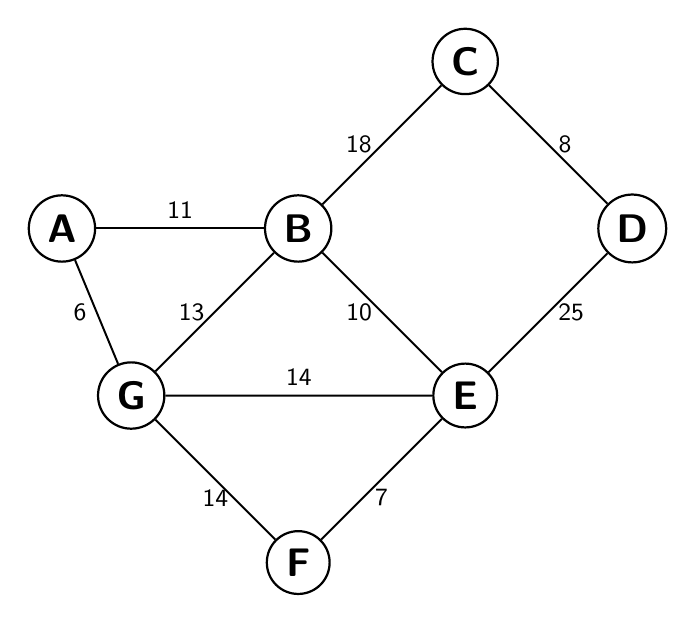
\begin{tikzpicture}[scale=0.4, auto, node distance=3cm, every loop/.style={},
  thick,main node/.style={circle,draw,font=\sffamily\Large\bfseries}]

\node[main node] (A) {A};
\node[main node] (B) [right of=A] {B};
\node[main node] (C) [above right of=B] {C};
\node[main node] (D) [below right of=C] {D};
\node[main node] (E) [below left of=D] {E};
\node[main node] (F) [below left of=E] {F};
\node[main node] (G) [above left of=F] {G};

\path[line width=0.25mm, every node/.style={font=\sffamily\small}]
(B) edge node [left]  {18} (C)
(B) edge node [left]  {10}  (E)
(C) edge node [right] {8}  (D)
(D) edge node [right] {25} (E)
(F) edge node [below] {14} (G)
(G) edge node [left]  {13} (B)
(G) edge node [above] {14}  (E)
(A) edge node [above] {11} (B)
(E) edge node [below] {7} (F)
(A) edge node [left] {6} (G)
;
\end{tikzpicture}
\end{center}
\end{required}


\begin{proof}[Answer]
\begin{itemize}
\item \textbf{Cite: adapted from Michaellevet's note.}
\item We initialize the intermediate spanning forest $\mathcal{F}$ to be the empty graph (the graph on no edges). We also
place the edges of G into a priority queue, which we call Q.\\ 
So: Q = [(\{A,G \},6), (\{E,F \},7), (\{C,D \},8), (\{B,E \},10), (\{A,B \},11), (\{B,G \},13), (\{E,G \},14), (\{F,G\},14), (\{B,C \},18), (\{D,E \},25)]

\item We poll from Q, which returns the edge \{A, G\}. Note that w(\{A, G\}) = 6. As A and G are on different
components of $\mathcal{F}$ (didn't result in a cycle), we \textbf{add} the edge \{B, C\} to $\mathcal{F}$.\\
So: Q = [(\{E,F \},7), (\{C,D \},8), (\{B,E \},10), (\{A,B \},11), (\{B,G \},13), (\{E,G \},14), (\{F,G\},14), (\{B,C \},18), (\{D,E \},25)]

\item We poll from Q, which returns the edge \{E, F\}. Note that w(\{E, F\}) = 7. As E and F are on different
components of $\mathcal{F}$ (didn't result in a cycle), we \textbf{add} the edge \{E, F\} to $\mathcal{F}$.\\
So: Q = [(\{C,D \},8), (\{B,E \},10), (\{A,B \},11), (\{B,G \},13), (\{E,G \},14), (\{F,G\},14), (\{B,C \},18), (\{D,E \},25)]

\item We poll from Q, which returns the edge \{C, D\}. Note that w(\{C, D\}) = 8. As C and D are on different
components of $\mathcal{F}$ (didn't result in a cycle), we \textbf{add} the edge \{C, D\} to $\mathcal{F}$.\\
So: Q = [(\{B,E \},10), (\{A,B \},11), (\{B,G \},13), (\{E,G \},14), (\{F,G\},14), (\{B,C \},18), (\{D,E \},25)]
 
\item We poll from Q, which returns the edge \{B,E\}. Note that w(\{B, E\}) = 10. As B and E are on different
components of $\mathcal{F}$ (didn't result in a cycle), we \textbf{add} the edge \{B, E\} to $\mathcal{F}$.\\
So: Q = [(\{A,B \},11), (\{B,G \},13), (\{E,G \},14), (\{F,G\},14), (\{B,C \},18), (\{D,E \},25)]

\item We poll from Q, which returns the edge \{A,B\}. Note that w(\{A, B\}) = 11. As A and B are on different
components of $\mathcal{F}$ (didn't result in a cycle), we \textbf{add} the edge \{A, B\} to $\mathcal{F}$.\\
So: Q = [ (\{B,G \},13), (\{E,G \},14), (\{F,G\},14), (\{B,C \},18), (\{D,E \},25)]

\item We poll from Q, which returns the edge \{B,G\}. Note that w(\{B, G\}) = 13. As B and G are on the same
components of $\mathcal{F}$ ( result in a cycle), we \textbf{do not add}  the edge \{B, G\} to $\mathcal{F}$.\\
So: Q = [ (\{E,G \},14), (\{F,G\},14), (\{B,C \},18), (\{D,E \},25)]

\item We poll from Q, which returns the edge \{E,G\}. Note that w(\{E, G\}) = 14. As E and G are on the same
components of $\mathcal{F}$ (result in a cycle), we \textbf{do not add} the edge \{E, G\} to $\mathcal{F}$.\\
So: Q = [ (\{F,G\},14), (\{B,C \},18), (\{D,E \},25)]

\item We poll from Q, which returns the edge \{F,G\}. Note that w(\{F, G\}) = 14. As F and G are on the same
components of $\mathcal{F}$ (result in a cycle), we \textbf{do not add} the edge \{F, G\} to $\mathcal{F}$.\\
So: Q = [ (\{B,C \},18), (\{D,E \},25)]


\item We poll from Q, which returns the edge \{B,C\}. Note that w(\{B, C\}) = 18. As B and C are on different
components of $\mathcal{F}$ (didn't result in a cycle), we \textbf{add} the edge \{B, C\} to $\mathcal{F}$.\\
So: Q = [ (\{D,E \},25)]

\item We poll from Q, which returns the edge \{D,E\}. Note that w(\{D, E\}) = 25. As D and E are on the same
components of $\mathcal{F}$ (result in a cycle), we \textbf{do not add} the edge \{D, E\} to $\mathcal{F}$.\\
So: Q = [ ]
\item As we have 7 vertex and 6 edges on $\mathcal{F}$, the algorithm terminates and return $\mathcal{F}$ as minimum-weight spanning tree. 
\end{itemize}
%Your answer goes here
\end{proof}



\newpage
\section{Standard 9- Prim's Algorithm}

\begin{required}
Consider the weighted graph $G(V, E, w)$ below. Clearly list the order in which Prim's algorithm, \textbf{using the source vertex} $A$, adds edges to a minimum-weight spanning tree for $G$. Additionally, clearly articulate the steps that Prim's algorithm takes as it selects the first \textbf{three} edges.

\begin{center}
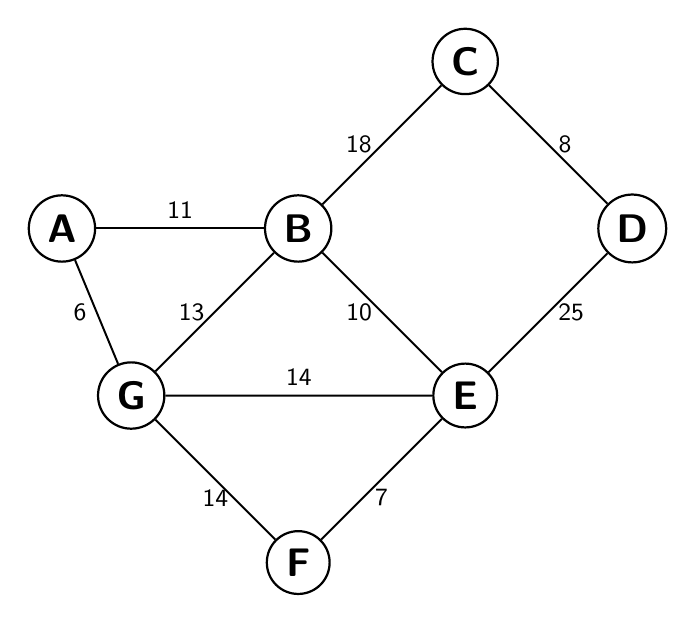
\begin{tikzpicture}[scale=0.4, auto, node distance=3cm, every loop/.style={},
  thick,main node/.style={circle,draw,font=\sffamily\Large\bfseries}]

\node[main node] (A) {A};
\node[main node] (B) [right of=A] {B};
\node[main node] (C) [above right of=B] {C};
\node[main node] (D) [below right of=C] {D};
\node[main node] (E) [below left of=D] {E};
\node[main node] (F) [below left of=E] {F};
\node[main node] (G) [above left of=F] {G};

\path[line width=0.25mm, every node/.style={font=\sffamily\small}]
(B) edge node [left]  {18} (C)
(B) edge node [left]  {10}  (E)
(C) edge node [right] {8}  (D)
(D) edge node [right] {25} (E)
(F) edge node [below] {14} (G)
(G) edge node [left]  {13} (B)
(G) edge node [above] {14}  (E)
(A) edge node [above] {11} (B)
(E) edge node [below] {7} (F)
(A) edge node [left] {6} (G)
;
\end{tikzpicture}
\end{center}
\end{required}


\begin{proof}[Answer]
%Your answer goes here
\begin{itemize}
\item \textbf{Cite: adapted from Michaellevet's note.}
\item The algorithm first initialize an intermediate spanning tree $\mathcal{F}$  with all the vertex in weighted graph G, but no edges in it. \\
Then, algorithm initialize an priority queue Q (ascending order) to contains the edge incident to the source vertex A.\\
So: Q:[(\{A,G \},6), (\{A,B \},11)]

\item Algorithm poll from Q and mark it as processed, which returns the edge \{A,G\}. Note that w(\{A, G\}) = 6. As A and G has exactly one end point on the component containing A (didn't result in a cycle), algorithm \textbf{add} the edge \{A,G\}  to $\mathcal{F}$. We then push into the priority queue the unprocessed edges incident to G (edges that not already in Q, and unprocessed )\\
So:  Q:[(\{A,B \},11), (\{B,G \},13), (\{E,G \},14), (\{F,G \},14) ]

\item Algorithm poll from Q and mark it as processed, which returns the edge \{A,B\}. Note that w(\{A, B\}) = 11. As A and B has exactly one end point on the component containing A (didn't result in a cycle), algorithm \textbf{add} the edge \{A,B\} to $\mathcal{F}$. We then push into the priority queue the unprocessed edges incident to B (edges that not already in Q, and unprocessed )\\
So:  Q:[ (\{B,E \},10), (\{B,G \},13), (\{E,G \},14), (\{F,G \},14), (\{B,C \},18), ]

\item Algorithm poll from Q and mark it as processed, which returns the edge \{B,E\}. Note that w(\{B, E\}) = 11. As B and E has exactly one end point on the component containing A (didn't result in a cycle), algorithm \textbf{add} the edge \{B,E\}  to $\mathcal{F}$. We then push into the priority queue the unprocessed edges incident to E (edges that not already in Q, and unprocessed )\\
So:  Q:[ (\{E,F \}, 7) (\{B,G \},13), (\{E,G \},14), (\{F,G \},14), (\{B,C \},18), (\{D,E \},25) ]

\item Algorithm poll from Q and mark it as processed, which returns the edge \{E,F\}. Note that w(\{E, F\}) = 11. As E and F has exactly one end point on the component containing A (didn't result in a cycle), algorithm \textbf{add} the edge \{E,F\}  to $\mathcal{F}$. We then push into the priority queue the unprocessed edges incident to F (edges that not already in Q, and unprocessed )\\
So:  Q:[ (\{B,G \},13), (\{E,G \},14), (\{F,G \},14), (\{B,C \},18), (\{D,E \},25) ]

\item Algorithm poll from Q and mark it as processed, which returns the edge \{B,G\}. Note that w(\{B, G\}) = 13. As both B and G  belong to the component containing A ( result in a cycle), algorithm \textbf{do not add} the edge \{B,G\} to $\mathcal{F}$. Then, nothing will be pushed into the Q.
So:  Q:[  (\{E,G \},14), (\{F,G \},14), (\{B,C \},18), (\{D,E \},25) ]

\item The algorithm \textbf{do not add} (\{E,G \},14) to $\mathcal{F}$, which result in a cycle if it is included. And both E and G belong to the component containing A\\
So:  Q:[  (\{F,G \},14), (\{B,C \},18), (\{D,E \},25) ]

\item  The algorithm \textbf{do not add} (\{F,G \},14) to $\mathcal{F}$, which result in a cycle if it is included. And both F and G belong to the component containing A\\
So:  Q:[ (\{B,C \},18), (\{D,E \},25) ]

\item  The algorithm \textbf{add} (\{B,C\},18) to $\mathcal{F}$ because B and C has exactly one end point on the component containing A (didn't result in a cycle). Then, We then push into the priority queue the unprocessed edges incident to C (edges that not already in Q, and unprocessed )\\ \\ 
So:  Q:[ (\{C,D \},8), (\{D,E \},25) ]

\item  The algorithm \textbf{add} (\{C,D\},8) to $\mathcal{F}$ because B and C has exactly one end point on the component containing A (didn't result in a cycle). Then, We then push into the priority queue the unprocessed edges incident to D (edges that not already in Q, and unprocessed )\\ \\ 
So:  Q:[ (\{D,E \},25) ]

\item  The algorithm \textbf{do not add} (\{D,E \},25) to $\mathcal{F}$, which result in a cycle if it is included. And both D and E belong to the component containing A\\
So:  Q:[  ]
\item Algorithm terminates, because we have $7$ vertex and $7-1 = 6$ edges in  $\mathcal{F}$. Then algorithm will return $\mathcal{F}$ as result.
\end{itemize}
\end{proof}
\end{document} % NOTHING AFTER THIS LINE IS PART OF THE DOCUMENT



